\documentclass[a4paper,12pt]{article} 
\usepackage[utf8x]{inputenc}
\usepackage[french]{babel}
\usepackage{mathtools}
\usepackage{amsmath, amssymb, amsfonts}
\usepackage{textcomp}
\usepackage[nointegrals]{wasysym}			% Collection de symboles mathématiques
\usepackage{ifthen}
\usepackage{tabularx}	 				% Gestion avancée des tableaux
\usepackage{longtable}		
%\usepackage{cleveref}

\usepackage{mathrsfs}

\usepackage{enumitem}
\usepackage{wrapfig}
%\usepackage[squaren]{SIunits}
%\usepackage[T1]{fontenc}				% Indispendable, présent dans tous les codes exemples
\usepackage[linkcolor=Indigo,colorlinks=true, citecolor=DarkSlateBlue, urlcolor=MidnightBlue]{hyperref} 	% Hyper ref
\usepackage{listings}					% Pour citer du code
\usepackage[justification=centering]{caption}
\usepackage{sistyle} 
\usepackage{numprint}
\usepackage{wrapfig}
\usepackage{cite}	
\usepackage{url} 					% Pour citer les sites internet dans la
%\usepackage{cleveref}
\usepackage{setspace}

\usepackage{graphicx}		 			% Inclusion des figures
\graphicspath{{./pic/}, {../figures/full_69_rapport/}}

\usepackage[svgnames]{xcolor}			%https://www.latextemplates.com/svgnames-colors


\usepackage{tikz} %Pour entourer un terme 
\newcommand*\circled[1]{\tikz[baseline=(char.base)]{
   \node[shape=circle,draw,inner sep=1pt] (char) {#1};}}
   
%%% Commandes utiles définies%
\newcommand{\argmin}{\mathop{\mathrm{argmin}}}

\newcommand{\bepar}[1]{
	\left( #1 \right)  
}

\newcommand{\becro}[1]{
	\left[ #1 \right]  
}

\newcommand{\beacc}[1]{
	\left\{ #1 \right \}  
}

\newcommand{\norm}[1]{
	\left \vert \left \vert #1 \right \vert  \right \vert
}

\newcommand{\rbk}[1]{\color{red}\textit{#1} \color{black}  
}

\usepackage{listings}					% Pour citer du code
%%%%%%%%%%%%%%%%%%%
%%% Élément pour citer des codes %%%
\lstset{
language=Python,
basicstyle=\ttfamily\bfseries\small, %
identifierstyle=\bfseries\color{black}, %
keywordstyle=\color{blue}, %
stringstyle=\color{black!90}, %
commentstyle=\it\color{black!70}, %
columns=flexible, %
tabsize=4, %
extendedchars=true, %
showspaces=false, %
showstringspaces=false, %
numberstyle=\small, %
breaklines=true, %
breakautoindent=true, %
captionpos=b,
otherkeywords={cross_val_score},
keywords=[0]{cv},
keywordstyle=[0]{\color{red}},
}
%%%%%%%%%%%%%%%%%%%%%
\title{\navy \textbf{Rapport CST fin première année} \color{black}}%%%%%%%%%%%%%%%%%%%%
\date{}
%\usepackage{multicol}
%\usepackage{etoolbox}
%\patchcmd{\thebibliography}{\section*{\refname}}
%    {\begin{multicols}{2}[\section*{\refname}]}{}{}
%\patchcmd{\endthebibliography}{\endlist}{\endlist\end{multicols}}{}{}
\usepackage[authoryear]{natbib}

\usepackage{geometry}
\geometry{hmargin=2cm, vmargin=1.8cm}

%%%%%%%%%%%%%%%%%%%%
%%% Couleurs %%%
\xdefinecolor{brick}{named}{DarkRed}
\xdefinecolor{navy}{named}{Navy}
\xdefinecolor{midblue}{named}{MidnightBlue}
\xdefinecolor{dsb}{named}{DarkSlateBlue}
\xdefinecolor{dgreen}{named}{DarkGreen}
\xdefinecolor{indian}{named}{IndianRed}

%%% 	Raccourcis 	%%%
\newcommand{\keps}{$k-\varepsilon$}
\newcommand{\covobs}{\text{C}^{-1}_{\text{obs}}}
\newcommand{\covpri}{\text{C}^{-1}_{\text{pri}}}
\newcommand{\bmap}{\beta_{\text{MAP}}}
\newcommand{\J}{\mathcal{J}}
\newcommand{\tinf}{$T_\infty$}
\newcommand\bk{\color{black}}
\newcommand\brick{\color{brick}}
\newcommand\navy{\color{navy}}
\newcommand\midblue{\color{midblue}}
\newcommand\dsb{\color{dsb}}
\newcommand{\dgreen}{\color{dgreen}}
\newcommand{\dpurple}{\color{indian}}
\newcommand\red{\color{red}}

%%%%%%%% Cigles
\newcommand{\rap}{par rapport}
\newcommand{\cad}{c'est-à-dire}
\newcommand{\vav}{vis-à-vis}
\newcommand{\NS}{Navier-Stokes}
\newcommand{\turb}{turbulence}
\newcommand{\inst}{instabilité}
\newcommand{\taur}{$\tau_{ij}$ }
%%%%%%%% Autres

%%%%%%%%%%%%%%%%%%%
% Syntax: \colorboxed[<color model>]{<color specification>}{<math formula>}
\newcommand*{\colorboxed}{}
\def\colorboxed#1#{%
  \colorboxedAux{#1}%
}
\newcommand*{\colorboxedAux}[3]{%
  % #1: optional argument for color model
  % #2: color specification
  % #3: formula
  \begingroup
    \colorlet{cb@saved}{.}%
    \color#1{#2}%
    \boxed{%
      \color{cb@saved}%
      #3%
    }%
  \endgroup
}

\renewcommand{\sectionmark}[1]{\markright{#1}}

\usepackage{fancyhdr}
\pagestyle{fancy}
\lhead{\textbf{Nathaniel} \brick \textbf{\textsc{Saura}}}
\rhead{\small Rapport première année}
%\rhead{\markright}
\cfoot{\thepage}
\renewcommand{\headrulewidth}{0.4pt}

\numberwithin{equation}{section} %%%% To count the equation like Section.Number

\usepackage{accents}
\newcommand{\vect}[1]{\accentset{\Rightarrow}{#1}}

\usepackage{multicol}		% Pour utiliser \hfill et découper une partie de son texte en colonnes
\setlength{\columnseprule}{0.1pt}
\def\columnseprulecolor{\color{red}}
\setlength{\columnsep}{1.5cm}

% Numéro Roman pour le texte
\makeatletter
\newcommand*{\rom}[1]{\expandafter\@slowromancap\romannumeral #1@}
\makeatother

\begin{document}
\begin{titlepage} \centering
\vspace*{\fill}
\Huge \navy \textbf{Rapport CST fin première année} \bk \normalsize
\vspace*{\fill}
\end{titlepage}
%\maketitle
%\end{center}
\newpage

\navy \section{Introduction du sujet}  \bk
\Large{$\mathscr{L}$}\normalsize a turbulence est l'état d'un fluide dont l'écoulement possède des caractéristiques stochastiques, qui passionne les chercheurs et les ingénieurs depuis plusieurs siècles.\\ 
Même si Léonard De Vinci au $\overline{\underline{\text{XV}}}^{\, \text{ème}}$ siècle avait mentionné ce caractère aléatoire et décrit quantitativement le phénomène par des observations, Osborne Reynolds en 1883 amorça la description qualitative et mathématique que nous utilisons aujourd'hui; il fut suivi par d'autres grands noms de la mécanique des fluides comme Richardson, Kolmogorov puis d'autres. \\
%Il construisit le nombre caractéristique dit de Reynolds qui compare les effets d'inertie et les effets visqueux. \\

\noindent Cette discipline est une des branches de la mécanique des fluides les plus actives qui attire énormément de chercheurs d'horizons plus ou moins éloignés de la mécanique des fluides ; Kolmogorov sus-mentionné était avant tout mathématicien.\\
Il existe de nombreux facteurs qui jouent sur la popularité de la discipline, sans être exhaustif, il est possible d'en développer deux : dans un premier temps cette théorie traite d'écoulement que l'on retrouve autour de soi dans notre vie de tous les jours (sillage d'une voiture, couche limite sur les ailes d'un avion etc...) mais également dans les océans, le ciel et l'espace. \\
Le deuxième facteur clé découle du premier : au fur et à mesure que de nouvelles technologies impliquant ce genre d'écoulement émergent, de l'intelligence provenant d'autres domaines de la Physique, de l'Informatique ou des Mathématiques devient nécessaire voire indispensable. \\

Au travers de ses équations, la théorie de la Turbulence entend modéliser les fluides dont les effets d'inerties ne sont pas négligeables devant les effets visqueux. Les équations de Navier-Stokes constituent la base de cette discipline. Si on considère une parcelle de fluide et que l'on y effectue un bilan de quantité de mouvement, on obtient dans un cas incompressible \footnote{Sans forces extérieures, avec $\rho$ la masse volumique (constante), $\nu$ la viscosité cinématique de l'écoulement et $p$  le champ de pression} :\\
\begin{equation}
\frac{\partial u_i}{\partial t} + \underset{\text{\red Inertie -  terme non linéaire \bk}}{\text{\red \circled{\bk $u_j\, \frac{\partial u_i}{\partial x_j}$}}} \bk = - \frac{1}{\rho} \frac{\partial p_i}{\partial x_j} + \underset{\text{\navy Visqueux \bk}}{\text{\navy \circled{\bk $\nu \frac{\partial^2 u_i }{\partial x_j^2}$}}} \bk 
%\tag{Navier-Stokes} 
\end{equation}
Les termes d'inerties ou de convection (nous considérons ici des flux ou des transports d'énergie mesurés en Watt) apparaissent dans le terme non-linéaire des équations de Navier-Stokes traduisant l'apport local d'énergie cinétique du fluide autour de la parcelle contrôlée.\\
Les effets visqueux traduisent la capacité du fluide à dissiper l'énergie de l'écoulement sous forme de chaleur.\\

Reynolds construisit un nombre sans dimension comparant les effets d'inertie sur les 
effets visqueux; il est appelé nombre de Reynolds, abrégé Reynolds; il peut s'écrire comme $$ \text{Re} = \bepar{u_j\, \frac{\partial u_i}{\partial x_j}} / \bepar{\nu \frac{\partial^2 u_i }{\partial x_j^2}} = \frac{\text{Effets inertiels} }{\text{Effets visqueux}} $$ \\
Ce nombre  caractérise l'état de l'écoulement. Pour un Reynolds faible (jusqu'à quelques centaines voire quelques miliers selon les cas), l'écoulement est dit laminaire. Lorsqu'il est au delà de la dizaine de milliers, l'écoulement est dit turbulent. \\
Entre les deux états, on parlera d'état de transition : des instabilités naissent dans l'écoulement rendant le champ de vitesse fluctuant. Plus le Reynolds augmente et plus ces fluctutations sont fortes, jusqu'à arriver à un champ de vitesse complétement aléatoire (turbulent). \\

Par analyse dimensionnelle, le nombre de Reynolds peut être construit comme le rapport 
\begin{equation}
 \text{Re} = \frac{\text{UL}}{\nu}
\end{equation} 
 La notion clé dans la théorie de la turbulence est que les échelles spatiales L, temporelles T et leurs combinaisons (comme la vitesse U = L/T) se décomposent en un nombre très élevé de sous-échelles.
Dans le cadre de la turbulence, on fera allusion au Reynolds des plus grandes échelles lorsqu'il sera question de nombre de Reynolds sans plus de précision sur l'échelle spatiale ou de vitesse. \\
Le passage du laminaire au turbulent est marqué par un changement topographique de l'écoulement. La première structure turbulente qui apparaît est en général un tourbillon dont les échelles caractéristiques sont similaires à celles du Reynolds «global». Sur ces échelles on pourra définir un temps caractéristique de retournement du tourbillon $\tau_{\text{retournement}} = L/U$. \\
Plus le Reynolds est grand et moins le fluide sera capable d'absorber les instabilités induites par l'inertie du fluide. En conséquence, à haut Reynolds, de l'énergie est constamment injectée dans la zone d'intérêt. Cette énergie est à l'origine de la multitude des échelles spatiales (et donc de toutes les autres) ; on parle de cascade\footnote{L'idée de cascade fut proposée par Richardson, mais sa description s'est avérée fausse. Kolmogorov en 1941 mis en évidence la casacade de Richardson de manière plus mathématique, sans pour autant utiliser cette appellation.} ou de brisure des échelles, \cad $ $ que l'énergie cinétique des premières structures de turbulence (à la suite d'instabilité) est distribuée de façon incohérente à des structures de taille plus petite. Ce processus est répété jusqu'à ce que le fluide soit capable de dissiper en chaleur l'énergie cinétique liées aux structures ainsi créées. \\

D'un point de vue pratique, les équations de \NS $ $ ne sont actuellement solubles «à la main» seulement pour des cas relativemenent simples. Pour la majorité des écoulements turbulents, il est nécessaire d'utiliser des outils numériques.\\
L'approche la plus précise pour résoudre ces équations est la méthode dite directe, ou DNS (Direct Numerical Simulation). Cette méthode entend résoudre les équations de \NS $ $ à toutes les échelles, et nécessite donc un maillage très resserré dans toutes les dimensions du problème, dont le pas est donnée par la théorie elle même. \\
Cette méthode est nécessite des ordinateurs très performants et plusieurs mois de calculs. Elle est souvent utilisée pour produire des résultats de référence pour être en mesure de critiquer les résultats de modèles numériques moins couteux et moins précis.\\
Dans un ordre de précision, les méthodes dites de LES (Large Eddy Scales) suivent les DNS. Schématiquement, cette catégorie de méthodes consiste à définir un seuil de prise en compte des échelles, accélérant ainsi les calculs. Pour assurer une prise en compte de la physique des plus petites échelles, la communauté utilisant ces méthodes construisent des modèles basés sur des termes modélisant la physique des échelles non prises en compte. Même si une partie des échelles est modélisée, ces méthodes restent fiables mais toujours 
trop lentes pour un usage en industrie.\\

 Enfin, il existe une dernière catégorie de méthodes consistant à construire des équations modélisant le(s) transport(s) de l'énergie cinétique turbulente $k$, du taux de dissipation de cette énergie $\varepsilon$, parfois les deux, ou parfois d'autres quantités (comme l'intermittence $\gamma$ ou la viscosité turbulente $\nu_T$). On parle de modèle à un ou deux équations; les plus connus sont le \keps, le Spalart-Allmaras et le $k-\omega$. Pour des raisons exposées plus tard, ces méthodes sont appelées méthodes RANS.\\
Ces modèles sont au cœur du travail effectué durant cette première année. Ils sont basés sur plusieurs idées propres à la théorie de la turbulence ou bien à leur construction.\\
 
\noindent Les designers de ces approches entendaient résoudre la turbulence uniquement pour les grandes échelles en modélisant les actions des autres échelles par des termes issus d'observations.\\
Les grandes échelles évoquées ici correspondent en fait au champ moyen de l'écoulement. En effet, une des idées de base de la théorie de la turbulence est la décomposition, dite de Reynolds. Elle consiste à écrire un champ turbulent en une somme d'une partie moyenne (temporelle) et d'une partie fluctuante. Les conventions variant d'un auteur à l'autre, dans le cadre de ce travail, les champs moyens seront écrits avec une barre au dessus (par exemple $\overline{U_i}$), les champs fluctuants seront écrits en minuscule.\\

Lorsque l'on injecte cette décomposition dans les équations de \NS $ $ sur la vitesse et la pression, on peut distinguer deux équations, une pour chacun des champs moyen et fluctuant. Pour plus de clarté, on écrit l'équation de \NS $ $ pour le champ moyen : 
\begin{equation}
 \frac{\partial \overline{U}_i}{\partial t} + \overline{U}_j \frac{\partial \overline{U}_i}{\partial x_j} = -\frac{1}{\rho} \frac{\partial \overline{P}}{\partial x_j} + \nu \frac{\partial^2 \overline{U}_i}{\partial x_j^2}  - \frac{\partial \, \overline{u_iu_j}}{\partial x_j} \label{meanfield}
 \end{equation}
  Cette équation est appelée RANS pour Reynolds Averaged \NS. On peut remarquer que le champ fluctuant agit directement sur le champ moyen l'évolution de ce dernier prend en compte un transport d'énergie associée à la partie fluctuante. Ce flux d'énergie représentée par le tenseur d'ordre deux $-\rho \overline{u_iu_j}$ est appelé tenseur de Reynolds. On le note $\tau_{ij}$.\\
Pour modéliser \taur, il est nécesaire de modéliser le tenseur d'ordre trois $-\overline{u_iu_ju_k}$ dont la modélisation nécessite celle du tenseur d'ordre quatre $-\overline{u_iu_ju_ku_l}$ et ainsi de suite. \\
Le fait de d'avoir besoin d'un tenseur d'ordre n+1 pour la modélisation de celui d'ordre n schématise la cascade sus-décrite et indique que les fluctuations aux différentes échelles sont fortement couplées.\\
  Il s'avère en fin de compte que le système formé des équations RANS et de celles du champ fluctuant est ouvert \cad $ $ qu'il y a plus d'inconnus que d'équations, il faut alors en rajouter une appelée l'équation de fermeture, c'est l'objet des méthodes à une ou plusieurs équation(s). L'effort dans ces approches et de simuler le terme de fluctuations pour obtenir le champ moyen, d'où l'appellation RANS.\\
  
  \noindent Dans ces méthodes RANS, on utilise l'hypothèse de Boussinesq. Celle-ci se base sur le fait que la création de nouvelles échelles augmente la stochasticité du champ de vitesse et donc de la friction au sein de l'écoulement.\\
  Il est alors proposé de construire un terme de viscosité liée à la turbulence à partir d'une analagie à la viscosité cinématique. La formule proposée par Boussinesq en 1890 s'écrit alors : 
\begin{equation}
\tau_{ij} = \rho \nu_T\bepar{\frac{\partial \overline{U}_i}{\partial x_j} + \frac{\partial \overline{U}_j}{\partial x_i}} - \frac{2}{3} \rho \overline{u_iu_i} \delta_{ij} \label{boussi}
\end{equation} 
   La quantité $\frac{1}{2}\overline{u_iu_i} $ est appelée énergie cinétique turbulente.\\La troisième idée que les méthodes dont il est question utilisent est d'utiliser des observations pour écrire des relations entre différentes quantités turbulente de l'écoulement. \\
Par exemple pour les modèles à deux équations \keps $ $ ou $k-\omega$ respectivement on utilisera une relation entre $k$ $\nu_t$ et $\varepsilon$ (resp. $\omega$). Des équations de transports modéliseront l'évolution (spatiale car ce sont des modèles stationnaires) de $k$ et de $\varepsilon$ (resp. $\omega$). Ces équations sont construites en injectant des constantes empiriques qui ont pour but de modéliser l'action (et les rétro-actions puisqu'il y a couplage) des petites échelles.\\

Pour les approches DNS les résultats corroborent exactement avec les résultats expérimentaux, la majeur contrepartie est le temps de calculs qui est encore très élevé malgré la parallélisation massive et l'utilisation de cluster d'ordinateurs. \\
Pour les méthodes LES et RANS les modélisations des effets de petites échelles ont tendance à perturber les résultats et impliquent une perte de précision. En revanche, pour des écoulements complexes les résultats sont bien plus probants avec l'approche LES que l'approche RANS.\\
Les méthodes RANS reposent beaucoup sur des constantes dont les valeurs sont déterminées par l'intuition, du réglages ou sur des valeurs standards définies à partir d'observations expérimentales sur une plage de cas peu variés, ou du moins non représentatif de la variété et la complexité des écoulements que l'on peut retrouver dans la nature.\\
Alors que les industriels n'utilisent en majorité que ce type d'approche afin de générer des résultats représentatifs rapidement, la question de la fiabilité des résultats se pose. En parallèle la théorie de la turbulence n'a que très peu avancé depuis les années 1980 et de nouvelles approches doivent être explorées comme il fut fait dans le passé.\\[2mm]

Au fur et à mesure que les méthodes numériques, les machines et les méthodes expérimentales se perfectionnaient, une quantité importante de données a pu être accumulée couvrant des écoulements classiques aux complexes, balayant des topologies variées et des spécificités propres aux différentes branches de la mécanique des fluides. Des méthodes ayant pour but d'utiliser ces données ont alors vu le jour, on parle de méthode pilotées par les données. Une des plus couramment utilisées est la méthode dite d'inversion : elle consiste à retrouver les paramètres d'un modèle, disposant auparavant des données issues de ce dernier et de ses variables d'états. \\

\noindent Cette méthode, dans sa philosophie, est en fait propre à l'élaboration de théories Physique. En effet, face à une situation (un écoulement, une onde se propageant...), les scientifiques réalisent des mesures de quantités d'intérêts, essaient de déterminer quelles sont les variables qui régissent le mieux le phénomène, établissent des équations en fonction des variables choisies et les quantités observées puis confrontent leur théorie avec les mesures réalisées en amont. 
Si la correspondance est bonne, la théorie est acceptée et testée dans d'autres cas. 
Si les équations ne rendent pas compte convenablement de la réalité, elles sont retravaillées. \\
On peut alors dire qu'intrinsèquement la Physique telle que nous la concevons a toujours été pilotée par les données disponibles et s'amèliorent avec les nouvelles observations expérimentales ou numériques. \\

\noindent Grâce au formalisme Bayesien (on parlera d'inférence Baysienne), il devient possible d'utiliser ce même procédé mais pour cette fois trouver les paramètres du modèle le moins précis (par exemple RANS ou LES) qui approcheraient le mieux les solutions de référence (DNS ou expériences).\\ 
Le procédé est le suivant : on injecte un terme optimisable dans les équations du modèles le moins précis, on évalue en chaque point la différence entre la solution fournie par ce dernier et la solution attendue (celle de référence), puis grâce à des méthodes d'opimisation on s'assure que le terme injecté corrige suffisamment bien cet écart jusqu'à atteindre le seuil voulu. \\
Ce procédé s'appelle la «maximalisation \textit{a posteriori}» de la fonction évaluant la probabilité d'obtenir le bon terme correctif sachant les observations disponibles.
Ainsi théoriquement, il devient possible de combiner rapidité de calcul et précision en «augmentant» les modèles RANS ou LES avec un terme correctif issu des données.\\
Cependant, cette inversion reste limitée par l'existence et la disponibilité de telles données, ce qui empêche la généralisation de cette même méthode.\\

La solution à ce problème fut également élaborée le siècle dernier. En effet, des méthodes d'apprentissage et de généralisation de pattern émergèrent. Une fois encore, la communauté scientifique saisit l'énorme (voire infini) potentiel de ces algorithmes avec l'amélioration des capacités des ordinateurs et la disponibilité des données.\\ L'ensemble de ces méthodes sont désignées aujourd'hui sous l'appellation d'intelligence artificielle (IA). Bien implémentées, ces méthodes permettent d'assimiler le processus liant les données entre elles et permettent sous certaines conditions de généraliser les données.\\

\noindent Depuis les années 2000, la recherche en Physique a vu l'incorporation toujours plus grande d'IA que ce soit pour améliorer la prédiction de modèles plus ou moins fiables, pour l'analyse de données, pour la détection de structures entre autres. \\
Avant d'entrer dans le vif du rapport, nous en présentons succintement le plan : le cœur de la première partie sera l'inférence et sa généralisation par réseau de neurones ou autres algorithmes. Les étapes du procédés seront détaillées ainsi que des résultats obtenu sur des problèmes différents. Les objectifs sur le court et le moyen terme seront également évoqués.\\
La deuxième partie se concentrera sur l'utilisation des réseaux de neurones comme seul outil de prédiction. Plusieurs remarques concernant le devenir de ces travaux au cours des deux prochaines années seront faites.\\
Dans une troisième partie plusieurs pistes d'études autour de ces thématiques seront abordées de manières plus brèves. L'accent sera porté sur l'origine de ces idées et sur l'importance qu'elles occuperont par la suite.

\pagebreak

\navy \section{Combiner vitesse et précision au travers l'association inférence et machine learning}
 \bk
\noindent Dans l'introduction générale de ce rapport, l'inférence et son principe ont été présenté superficiellement pour pouvoir introduire la notion de méthode pilotée par les données. Nous proposons ici de rentrer plus en détail dans la théorie et dans son utilisation. \\
Dans l'ensemble de ce rapport, $\beta$ est un vecteur.
\brick \subsection{Présentation de l'inférence et de ses outils} \bk
\dsb \subsubsection{Théorème de Bayes et fonction de correspondance} \bk
L'inférence Bayesienne se base sur le théorème de Bayes établit fin du $\overline{\underline{\text{XVIII}}}^{\, \text{ème}}$ siècle. Il permet d'évaluer une distribution de probabilité des paramètres que l'on cherche à évaluer, sachant les observations ou les mesures.\\
Dans l'étude présentée, le paramètre recherché est un vecteur noté $\beta$, les observations seront notés \textbf{d}. Le théorème de Bayes permettra d'évaluer la probabilité $p\bepar{\beta\,|\,d}$; il établit 
\begin{equation}
p\bepar{\beta\,|\,\textbf{d}} = \frac{\mathcal{L}\bepar{\textbf{d}\,|\,\beta}p\bepar{\beta}}{c} %\tag{Théorème de Bayes}
\end{equation}
Ce théorème lie la probabilité d'obtenir les observations sachant un premier essai de $\beta$ (on parlera d'information \textit{à priori}) $\mathcal{L}\bepar{\textbf{d}\,|\,\beta}$, avec la distribution \textit{a priori} du vecteur $\beta$, $p\bepar{\beta}$. Le premier terme est appelée distribution de correspondance ou \textit{likelihood distribution} $\mathcal{L}$.\\
Au dénominateur, le terme $c$ représente la \textit{likelihood marginalisée} par tous les paramètres possibles. Le but étant de construire une moyenne de $\mathcal{L}\bepar{\textbf{d}\,|\,\beta}$ par rapport aux choix de paramètres à priori. $c$ s'écrira donc 
\begin{equation}
c = \int_{\beta} \mathcal{L}\bepar{\textbf{d}\,|\,\beta}p\bepar{\beta} d\beta
\end{equation} \\
Calculer $p\bepar{\beta\,|\,\textbf{d}}$ peut se faire en supposant que \textbf{d}, $\beta$ et $\mathcal{L}$ ont des distributions gaussiennes comme suggéré par \citep{parish2016paradigm} \citep{aster2011parameter} ou encore \citep{tarantola2005inverse}.\\
La méthode MAP pour \textit{Maximum A Posteriori} utilisée par les références citées, consiste à calculer la valeur de $\beta$ la plus probable plutôt que de déterminer de l'entière distribution. L'objectif est alors de maximiser la correspondance entre modèle et observation soit 
\begin{equation}
\beta_{\text{MAP}} = \underset{\beta}{\text{arg}\, \text{max}} \ p\bepar{\beta\,|\,\textbf{d}} \label{bmap}
\end{equation}
À partir de développement mathématique qui ne seront pas mentionnés ici, il est possible d'écrire $\mathcal{L}$ comme une fonction de coût. Souvent les données expérimentales sont obtenues avec une incertitude propre à la méthode de mesure ou aux outils utilisés. Ces incertitudes devant apparaître, on construit une matrice de covariance $\covobs$ (nous n'utiliserons que son inverse). \\
Idem, puisque $\mathcal{L}$ prend en compte la première valeur (premier choix ou first guess) $\beta_{\text{pri}}$ et sa distribution, la fonction de coût équivalente doit faire apparaître la covariance $\covpri$.\\
Finalement avec $\textbf{h}_\beta \equiv \textbf{h}(\beta)$ la prédiction du modèle qu'on essaie de corriger, effectuer une inversion revient à estimer 
\begin{equation}
\bmap = \underset{\beta}{\text{arg}\, \text{min}}\ \frac{1}{2}\becro{\bepar{\textbf{d} - \textbf{h}_\beta}^T \covobs \bepar{\textbf{d} - \textbf{h}_\beta} + \bepar{\beta - \beta_{\text{pri}}}^T \covpri  \bepar{\beta - \beta_{\text{pri}}}} \label{bmapJ}
\end{equation}
La fonction à minimiser est la fonction de coût sus-mentionnée, elle est notée $\mathcal{J}$ dans la suite.

\dsb \subsubsection{L'algorithme BFGS} \bk

\noindent La résolution de ce problème devient alors un problème de minimisation. Nous utilisons l'algorithme Broyden-Fletcher-Goldfarb-Shanno abbrégé BFGS dans la suite \citep{nocedal2006numerical}.
Contrairement aux Algorithmes de gradient classiques, le BFGS est un algorithme d'ordre deux. Il utilise une une approximation de la hessienne de $\J$ afin de ne pas avoir à effectuer le calcul de cette matrice qui peut s'avérer très lourd.\\
C'est une méthode itérative mettant à jour le vecteur d'intérêt $\beta_k$ ainsi que sa hesienne inverse notée $B^{-1}_k$ à partir d'un algorithme d'exploration appelé \textit{line search} dont nous évoquerons brièvement les spécificités.\\
Pour atteindre le minimum global de l'équation \eqref{bmapJ}, il est nécessaire d'incrémenter la valeur de $\beta_k$ par une variation $d\beta_k$ vérifiant l'inégalité suivante
\begin{equation}
\nabla\J_k = \frac{\partial \J}{\partial \beta_k} = \frac{\J\bepar{\beta_k+ d\beta_k} - \J\bepar{\beta_k}}{d\beta_k} < 0
\end{equation}
Pour déterminer la forme de cet incrément le BFGS procède en deux étapes : dans un premier temps l'algorithme détermine la \textit{direction} du gradient puis la \textit{longueur} de l'incrément. \\
On note le vecteur de direction $\mathbf{p}_k$, il s'écrit :
\begin{equation}
\mathbf{p}_k = -B_k^{-1}\nabla_k\J
\end{equation}
Pour vérifier que ce vecteur pointe dans la bonne direction, le produit scalaire du gradient $\nabla_k\J$ projeté sur la hessienne doit vérifier l'inéquation:
\begin{equation}
-\nabla_k^T\J\, B_k^{-1}\, \nabla_k\J = \mathbf{p}_k^T\, \nabla_k\J < 0
\end{equation}
Cette condition est une conséquence directe du développement de Taylor autour de l'incrément.\\

\noindent Une fois la direction calculée, il reste à déterminer l'amplitude de l'incrémentation. En effet, puisque l'on cherche le minimum global de $\J$, il faut veiller à ne pas «tourner autour» du $\bmap$ indéfiniment, et adapter le pas au fur et à mesure que l'optimisation se déroule.\\ 
Sans rentrer dans dans tous les détails, le BFGS utilise un algorithme de \textit{line search} pour trouver $ \displaystyle \alpha_k$ tel que $d\beta_k = \alpha_k\mathbf{p}_k$. Cette recherche doit satisfaire deux critères sur $\beta_{k+1}$: 
\begin{itemize}
\item[$\bullet$] Une condition sur la nouvelle valeur de la fonction de coût : \begin{equation}
\J\bepar{\beta_{k+1}} - \J\bepar{\beta_k} < C_1
\end{equation} 

\item[$\bullet$] Une condition sur la pente (ou la courbure) : 
\begin{equation}
|\nabla(\beta_{k+1})|^T\textbf{p}_k < C_2 |\nabla_k^T\textbf{p}_k|
\end{equation}
\end{itemize} 
$C_1$ et $C_2$ étant deux seuils préalablement définis.\\
La dernière étape de l'algorithme consiste à incrémenter $B_{k+1}^{-1}$ utilisant $\alpha_k$ ainsi que d'autres termes construit à partir de $\beta_{k+1}$.\\

\pagebreak

\brick \subsection{Utilisation de l'inférence sur différents cas} \bk

Nous avons mis en place les outils présentés ci-dessus dans plusieurs cas, nous n'en présenterons que deux : un problème thermique monodimensionnel provenant de \citep{parish2016paradigm}, puis sur la propagation d'une onde à travers l'équation de Burgers 1d.

\dsb \subsubsection{Problème thermique} \bk
Le but est d'établir l'évolution du champ de température dans un barreau dont les températures au début et en fin de domaine sont nulles. Cette évolution se fait sous des termes de conduction, de convection et de radiation. Le paramètre de ce problème sera la température extérieure au barreau $T_\text{inf}$. 
L'équation exacte qui régit ce problème s'écrit 
\begin{equation}
 \frac{d^2T}{dz^2} + \varepsilon(T)\bepar{T^4_\infty - T^4} + h\bepar{T_\infty - T} = 0 \label{Ttrue} \tag{EE}
 \end{equation} 
 Avec 
 \begin{equation}
 \varepsilon(T) = \becro{1 + 5 \sin\bepar{\frac{3\pi}{200}\, T} + \exp\bepar{0.02\,T}+ \mathcal{N}\bepar{0,\, 0.1^2}} \times 10^{-4} \label{epsilon}
 \end{equation}
 On commence par résoudre ce problème exact pour plusieurs tirage de $\varepsilon$. On utilise a méthode de Crank-Nicholson pour résoudre ce problème, en ajoutant artificiellement un terme d'évolution temporelle.\\
 En même temps de construire une dataset de référence, on évalue la sensibilité des résultats par rapport à la distribution $\mathcal{N}$ présente dans l'équation \eqref{epsilon}. Cette sensibilité se traduit par la construction d'une matrice de covariance des données observables issues de ce problème exact.\\
 Afin de tester l'inférence, nous biaisons l'équation exact \eqref{Ttrue} et établissons un problème inexacte (E$\beta$) :
\begin{equation}
\frac{d^2T}{dz^2} + \varepsilon_0\beta(z)\bepar{T^4_\infty - T^4}= 0 \tag{E$\beta$} \label{Tinex}
\end{equation}
Nous construisons $\covpri$ en diagonalisant des valeurs fournies par \citep{parish2016paradigm}.\\

Au cours de la minimisation,  afin de pouvoir voir la solution se dessiner, il a été nécessaire de coder un solver BFGS en suivant \citep{nocedal2006numerical}. Un exemple de cette évolution pour \tinf = $50$ est illustrée Fig.\eqref{tinf50}.\\
Le critère de convergence est ici une condition sur $||\nabla_{\beta_k}\J||_\infty$ ou bien sur un nombre limite d'itérations. La figure Fig.\eqref{s} récapitule l'évolution de cette grandeur en cours d'optimisation.\\
\indent La méthode BFGS permet également d'avoir accès à la hessienne inverse de $\J$ évaluée sur $\bmap$. Grâce à sa décomposition de Cholesky, on peut construire une approximation de la distribution $p\bepar{\beta\,|\,\textbf{d}}$ autour de $\bmap$. \\
On note $R$ tel que $\text{Chol}\bepar{B_{\bmap}^{-1}} = \text{R}\text{R}^T$ et $s \sim \mathcal{N}\bepar{0,1}$. Ainsi 
\begin{equation}
p\bepar{\beta\,|\,\textbf{d}} \approx \bmap + \text{R}s
\end{equation}
Il devient possible d'évaluer la variance de cette distribution. Sur 250 tirages de $\beta$, on résout \eqref{Tinex}, on calcule les extrema ainsi que les déviations standards. On fait de même avec $\bmap$ solution de l'optimisation de scipy, et l'on compare les extrema sur chacun des points du domaine; disposant d'une écriture analytique pour $\beta_{\text{True}}$, on peut évaluer la fiabilité de la méthode en traçant toutes ces grandeurs dans une même figure voir Fig.\eqref{s}: 

\begin{figure}[!ht]
\centering
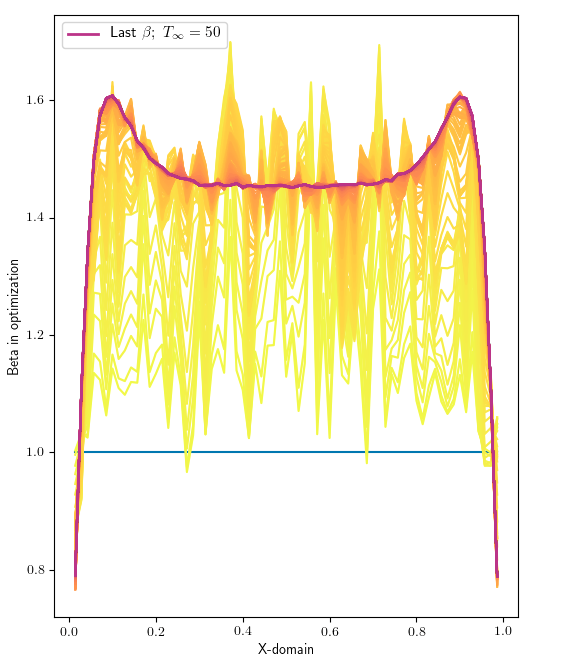
\includegraphics[scale=0.52]{Just_bmapTinf50.png}
\caption{À gauche évolution de beta au cours de l'optimisation pour $T_\infty$. La droite bleue représente le first guess de $\beta$. Plus la teinte est foncée plus on se rapproche de $\bmap$.}
\label{tinf50}
\end{figure}

\dsb \subsubsection{Propagation d'une onde en fluide visqueux} \bk
L'équation de Burgers permet d'étudier la propagation des ondes et peut faire apparaître des chocs. Nous voulons dans un premier temps déterminer si l'inférence peut capturer les chocs. Dans un second temps, nous voulons déterminer si ce genre de méthode permet de capturer les non-linéarités. \\
Notons que cette démarche s'inscrit dans un projet plus vaste : utiliser une combinaison de méthode pilotée par les données et de machine learning pour construire un modèle de différences finies augmentées dépassant les capacités des méthodes de différences finies classiques.\\

\noindent Contrairement au cas précédent, l'équation de Burgers est instationnaire. Il a fallu alors écrire un code qui réalise une inférence à chaque itération temporelle. Le principe de l'inférence, la façon dont elle est réalisée et son objectif sont les mêmes que décrits plus haut.\\

\noindent L'équation de Burger visqueuse (VBE) s'écrit 
\begin{equation}
\frac{\partial u}{\partial t} + u \frac{\partial u}{\partial x} = \nu\frac{\partial^2 u}{\partial x^2}  \label{VBETrue} \tag{VBE}
\end{equation}
Nous résolvons cette équation en utilisant le schéma de Lax-Wendroff. La condition initiale est est un sinus de déphasage nulle, aniti-symétrique par rapport au centre du domaine.\\
Comme précédemment, il nous faut approximer cette équation avec un terme $\beta$ modélisant un des termes de l'équation précédente. Nous remplaçons ici le terme non-linéaire de convection $\displaystyle u \frac{\partial u}{\partial x}$. On définit alors

\begin{equation}
\frac{\partial u}{\partial t} + u \beta(x,t) = \nu \frac{\partial^2 u}{\partial x^2} \label{VBEbeta} \tag{VBE$\beta$}
\end{equation}
L'équation précédente est linéaire en $u$ alors que l'équation \eqref{VBETrue} ne l'est pas.\\
On définit la fonction de coût en comparant les solutions de ces deux équations. Si $n$ est l'itération courante, ajuster $\beta_n$ nécessite donc d'évaluer l'écart entre les solutions exactes et inexactes à l'itération $n+1$.\\
Pour éviter toutes ambiguïtés, on précise les indices dans la fonction de coût suivante 
\begin{equation}
\mathcal{J}^n = \frac{1}{2} \bepar{\Delta_{_{\text{LW-CN}}}U^{n+1}}^T \text{C}_\text{obs}^{-1} \bepar{\Delta_{_{\text{LW-CN}}}U^{n+1}} + \lambda \bepar{\beta^n -
			\beta_{\text{p}}}^T \text{I}_d \bepar{\beta^n - \beta_\text{p}}
\end{equation}
Avec 
\begin{equation}
\Delta_{_{\text{LW-CN}}}U^{n+1} = \bepar{U^{n+1}_{\text{obs}}}^\text{LW} - \bepar{U^{n+1}_\beta}^\text{CN}
\end{equation}
De façon similaire, $\bmap^{n}$ sera obtenu en résolvant un problème d'optimisation :
\begin{equation}
\beta_{\text{MAP}}^n = \argmin \mathcal{J}^n
\end{equation}
Il est nécessaire de vérifier si les solutions sont similaires à toutes les itérations. Dans la figure suivante, une comparaison aux itérations 30 et 35 (sur 50) des champs $u^n_{\text{True}}$ et $u^n_{\beta}$ sont présentées. 

\begin{figure}[!ht]
\vspace{-5mm}
\centering
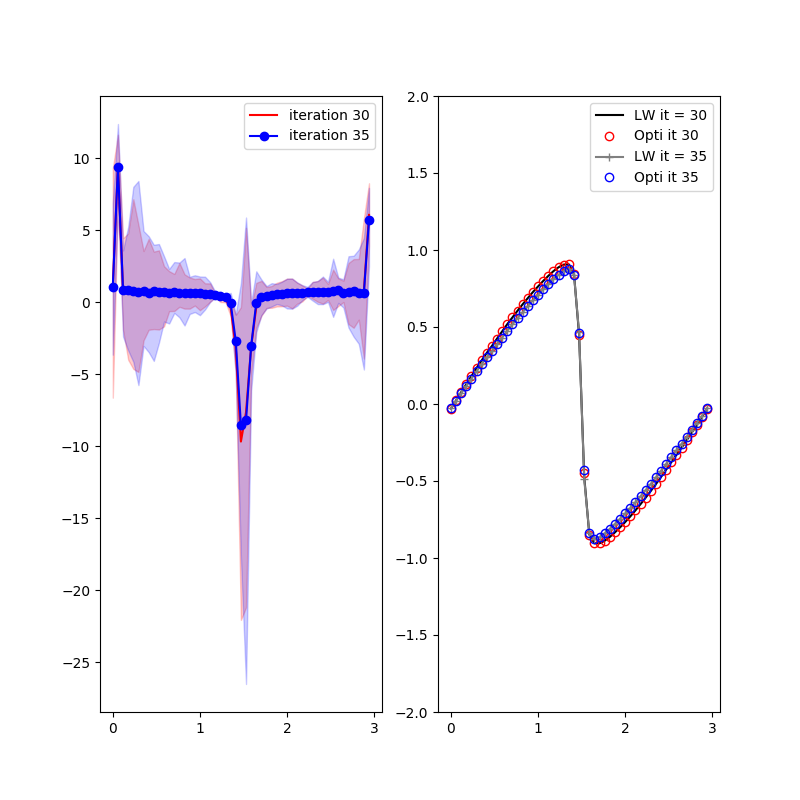
\includegraphics[scale=0.7]{nu0_0250_CFL0_40_Nx_52_InferenceVSTrue_it35.png}
\caption{}
\label{}
\end{figure}

Les zones opaques représentent les variations possibles des distributions des $\bmap$. Leurs amplitudes assez grandes proviennent du fait qu'un nombre d'itérations maximales assez faible à été imposé lors de la minimisation.\\ 
Toujours est il que la superposition est parfaite pour toutes les itérations et qu'on a prouvé que l'inférence pouvait être utilisée même dans des cas instationnaires.\\
Le choc est bien capturé et la dissipation par effet visqueux dans la suite de la simulation est également parfaitement retrouvée.\\

\noindent Dans cette thèse, mettre en place une procédure d'inférence n'est pas une fin en soi, mais une étape qu'il était indispensable de maîtriser pour l'atteinte des objectifs visés.\\
Comprendre le formalisme mathématique de cet outil, avec la fonction de correspondance $\mathcal{L}$, l'optimisation de paramètres $\beta$ pour faire correspondre modèle et observations, permet d'avoir une première approche des algorithmes d'entraînement des intelligences artificielles comme le réseau de neurones.\\
En effet, les algorithmes de machine learning (ML) fonctionnent sur un principe très similaire à celui de l'inférence Bayesienne puisqu'ils cherchent à ajuster plusieurs paranmètres (parfois des milliers voire des millions) afin de faire correspondre des entrées (\textit{input)} à des sorties, toutes les deux fournies par l'utilisateur; c'est ce qu'on appelle l'entraînement ou \textit{learning}. Une fois ces paramètres établi, ces méthodes entendent prédire des sorties à partir d'entrées inédites, c'est ce qu'on appelle la prédiction.\\
L'idée de généraliser les données de l'inférence par ML est donc de d'apprendre la fonctionnelle qui existe entre les caractéristiques d'un problème et le vecteur $\bmap$ calculé au préalable sur plusieurs cas, afin de pouvoir prédire dans des cas inédits le bon vecteur de correction.\\

\brick \subsection{Les réseaux de neurones} \bk
%En parallèle, notre ère connait une hausse de l'utilisation d'algorithmes d'intelligence artificielle (IA) ou d'élaboration de procédés de résolution de problème pilotées par les données; et le nombre d'articles sur ces thèmes ainsi que leurs applications pratiques explosent. L'idée majeur de ce genre de méthode est le fait qu'on peut découvrir de l'information au sein des données afin de les généraliser (dans le cas d'IA.) ou de s'en servir pour corriger les prédictions de modèles peu fiables (dans le cas des méthodes pilotées par les données).\\
%Appliqués aux problématiques de la turbulence, ces algorithmes pourraient par exemple aider à identifier les régions ou les modélisations RANS ne sont pas fiables \citep{ling2015evaluation}, tirer le meilleure de résultats algébriques comme ceux de \citep{pope1975more} pour élaborer des modèles RANS augmentés par une IA type réseaux de neurones ou forêt aléatoire \citep{ling2016machine}.\\
%À partir de méthodes type inférence baysienne, on peut également construire des méthodes utilisant la structure de modèles RANS à une ou deux équations en injectant un vecteur de correction d'une itération à l'autre en comparant avec des cas dont les résultats DNS ou expérimentaux sont connus c'est en partie le travail effectué par \citep{singh2017machine}, \citep{parish2016paradigm} ou encore \citep{tracey2015machine} pour ne citer que quelques travaux.\\

%\href{./objectif.pdf}{This is my link}

   
\pagebreak

\bibliographystyle{apalike}
\bibliography{bibliotheque}


\end{document}